\section{Literature Review}
In this section the following (sub-)research questions are answered to get an overview of the current state-of-the-art of Distributed Machine Learning:
\begin{itemize}
	\item What are the advantages of Distributed Machine Learning over (centralized) Machine Learning?
	\item What technology is used for Distributed Machine Learning?
	\item What are the currently used implementations?
\end{itemize}

\subsection{The need for Distributed Machine Learning}
.
\subsubsection{Alternatives to Distributed machine learning}
The most popular solution to increasing computation power for Machine
learning is currently distributing the workload over a large amount of machines. However, there are other, more traditional ways to increase the available computation power. Such as the use of dedicated Graphics processing units (GPUs), the use of Application Specific Integrated Circuits (ASICs) or special multi-core computer architectures.

\paragraph{GPUs in Machine Learning}
The use of GPUs in machinlearning is already a very common method. This is due to the nature of the data which makes up machine learning problems. A GPU is extremly fast at making multiple small calculations on a batch of data. Luckily the data that is requiered by Machine Learning algorithms such as Neural Networks and Unsupervised Learnign is of this type. This means that GPUs have had alot of succes with speeding up these calcultions as was found by Meuth \ref{Meut2007} who reported a up to 200x speed up over conventional CPUs.


\paragraph{Application Specific Integrated Circuits}
The idea of using Application Specific Integrated Circuits (ASICs) in highly specialized tasks is not new to Machine Learning. In recent times, the demand for such chips has risen massively\cite{Metz18}.
When applied to e.g. Bitcoin mining, ASICs have a significant competitive advantage over GPUs and CPUs, which achieve only a fraction of the performance per watt. The expectations of ASICs are high in the context of Machine Learning as well, because many of the computations involved come in the form of matrix multiplications. This is an area in which some ASICs excel.

Google applied this concept in their own Tensor Processing Unit (TPU)\cite{Sato17}, which, as the name suggests, is an ASIC that specializes in calculations that use tensors ($n$-dimensional arrays). The TPU works well when combined with their Tensorflow\cite{Tensorflow2015}\cite{Tensorflow2016} framework, which is one of the most popular building blocks for Machine Learning models.

The most important component of the TPU is its Matrix Multiply unit, which is what differentiates the chip from a CPU/GPU. The TPU can be connected to a server over a PCI-e bus. Many TPUs can be used in a data center, and if the work load is high even for a TPU, multiple units can collaborate in a distributed setting.

The performance improvement of the TPU over regular CPU/GPU setups is not only because of its increased processing power, but also its power efficiency, which is important for large companies that want to minimize energy costs. When running benchmarks, \citet{Joup17} found that the performance per watt of a TPU can approach 200x that of a traditional system.

Further benchmarking by \citet{Sato17} indicated that the total processing power of a TPU or GPU can be up to 70x higher than a CPU in a standard Neural Network, with performance improvements varying from 3.5x - 71x depending on the task at hand.


\paragraph{Computer architectures}
Other than using ASICs in order to increase the amount of work a computer can do,
general-purpose processors can also be built with different architectures that significantly increase the number of usable cores. Such an architecture exists in the form of Epiphany. It is a Multiple Instruction, Multiple Data (MIMD) architecture that uses an array of processors, each of which accessing the
same memory, to speed up execution of floating point operations\cite{Olof16}.

The newest chip of the major manufacturer Adapteva is the Epiphany V, which contains
1024 cores on a single chip\cite{Olof16}. Although Adapteva has not published power consumption specifications of the Epiphany V yet, it has released numbers boasting a power usage of only 2 watt\cite{Adap}.

Using multiple processors to process a single dataset is not a new idea in Computer Science. Message Passing Interface (MPI)\cite{MPI1993} was developed to simplify the distribution of work for this purpose, and is usually applied on a cluster of workers. The same framework, however, can also be adapted to the Epiphany chips, as was demonstrated by \citep{Rich15}. They found that the RISC chips were able to perform matrix operations rapidly until their on-board memory was filled.

\paragraph{Future relevance}
As can be seen in the examples above, there are many different strategies to obtain the processing power needed for large-scale Machine Learning. These techniques focus both on power efficiency and raw computational power. However, it must be noted that distributed systems are often preferred to these non-distributed alternatives above a certain scale, because of higher scalability and lower equipment cost. The techniques described above can still be used in a distributed setting, without suffering major performance degradations. This makes them a good choice for certain classes of future applications, as they can provide the benefits of optimized hardware in a distributed system.










\subsection{Underlying technology}
To give you an overview of how Distributed Machine Learning works, we'll give you an abstract framework that includes everything a real implementation should include, see Figure \ref{overview_system}.\\
\begin{figure}[H]
	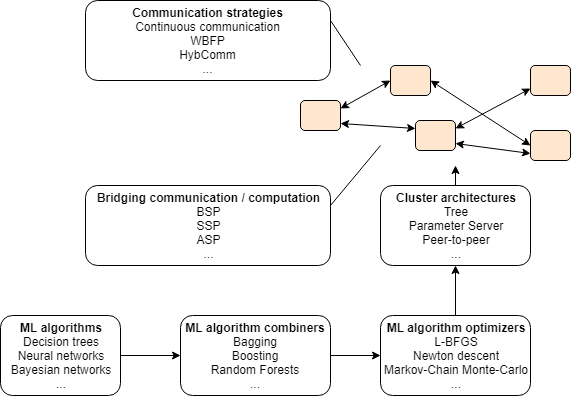
\includegraphics[width=\textwidth]{general_system_bac_sem.png}
	\caption{An overview of the algorithms that make up our general system for Distributed Machine Learning}
	\label{overview_system}
\end{figure}
This system exploits three unique properties of Distributed Machine Learning: error tolerance, dynamic structural dependencies, and non-uniform convergence.\cite{Xing16}\\
Our goals include (1) to list regular Machine Learning algorithms that are commonly used in a distributed setting; (2) to find algorithms to determine the best parameters for the aforementioned algorithms; (3) to find a balance between computation time, communication overhead, and accuracy; and (4) to minimize the number of bits sent over the network, so that the system is not bottlenecked by network bandwidth.\\
Designing a generic system that enables distribution of  regular Machine Learning efficiently is challenging, because every algorithm has its own communication patterns \cite{Jia14}\cite{Newman09}\cite{Rich13}\cite{Smola10}\cite{Takac13}\cite{Tsi12}.

\subsubsection{Machine Learning algorithms}
Machine Learning algorithms learn to make predictions or decisions based on data. Every Machine Learning algorithm has its own pros and cons. Machine Learning algorithms can be divided into categories based on some of their characteristics:
\begin{itemize}
	\item \textbf{Feedback}, the type of feedback that is given to the algorithm while learning
	\item \textbf{Goal}, the type of output that is generated
	\item \textbf{Type}, the architecture used to generate output
	\item \textbf{Method}, the nature of model evolution that occurs when given feedback
\end{itemize}

\paragraph{Feedback}
\begin{itemize}
	\item \textbf{Supervised}
		learning uses training data that consists of input objects (usually vectors) and output values. Supervised learning algorithms typically attempt to find a function that maps input data to some output. They then apply this function to find outputs for unknown input data.
		% bias vs variance
		% complexity vs amount of data
		% dimensionality
		% noise
	\item \textbf{Unsupervised}
		learning uses unlabeled training data. It therefore lacks a clear output accuracy metric. Common use cases are clustering and pattern recognition.
	\item \textbf{Semi-supervised}
		learning uses a (generally small) amount of labeled data, supplemented by a comparatively large amount of unlabeled data. Clustering can be used to extrapolate known labels onto unlabeled data points. This is done under the assumption that similar data points share a label.
	\item \textbf{Reinforcement learning}
		relies on a secondary feedback system that evaluates the output accuracy of the model being trained. The feedback system either minimizes a risk function or maximizes a reward function. Reinforcement learning therefore doesn't require a big dataset of correct and incorrect input-output pairs. Because of the black box behavior of the model, it is not possible to explicitly correct actions that are sub-optimal. As a result, the model can converge on a local minimum.
		% Q-learning
\end{itemize}

\paragraph{Goals}
\begin{itemize}
	\item \textbf{Anomaly detection}
		can be divided into 3 categories. \textbf{Supervised anomaly detection} requires data that has a different label for abnormal data, on which it trains a classifier. \textbf{Unsupervised anomaly detection} assumes that normal and abnormal data points are separable, and clusters them. \textbf{Semi-supervised anomaly detection} builds a model of normal data, and tests whether new data points are normal or abnormal. Which of these categories is best depends on dataset characteristics.
	\item \textbf{Classification}
		is the problem of categorizing unknown data points into categories seen during training. This is an inherently supervised process; its unsupervised equivalent is clustering.
	\item \textbf{Clustering}
		is the problem of grouping together data points that are similar according to some metric. This can be solved through supervised learning, but is usually done with large datasets, for which labeling might be expensive.
	\item \textbf{Dimensional reduction}
		is the problem of reducing the number of variables in the input data. This can either be achieved by selecting only relevant variables (\textbf{Feature selection}), or by creating new variables that represent multiple others (\textbf{Feature extraction}).
	\item \textbf{Feature learning / Representation learning}
		is the problem of finding proper representations of input data for e.g. feature detection, classification, clustering, encoding, or matrix factorization.
		% manifold learning
		% statistical inference/density estimation
		% sparse coding
	\item \textbf{Regression}
		is the problem of estimating how dependent variables relate to their dependencies. Parametric regression attempts to encode this in parameters of some function, which speeds up the process if, for example, a linear correlation is expected. Nonparametric regression constructs a predictor according to information derived from the data. It does this without relying on a predetermined form. This requires a larger sample size and significantly more time.
\end{itemize}

\paragraph{Types}
\begin{itemize}
	\item \textbf{Evolutionary algorithms (EAs)} (and 
		specifically \textbf{Genetic algorithms}) learn iteratively based on evolution. The algorithm that actually solves the problem is represented by a set of properties, called its \textbf{genotype}. The performance of the algorithm is measured using a score, calculated using a \textbf{fitness function}. After calculating the fitness score of all generated algorithms, the next iteration creates new genotypes based on mutation and crossover of algorithms that are produce more accurate estimates. Generic algorithms can be used to create other algorithms, such as neural networks, belief networks, decision trees, and rule sets.
	% Graphical models
	\item \textbf{Perceptron-based}
		algorithms use binary classifiers (Perceptrons) that label input vectors as 'active' or 'inactive'. Perceptrons assign a weight to all inputs. It then sum over the products of these weights and their input. The outcome of this is compared to a threshold (known as the \textbf{bias}) to determine the label. Perceptron-based algorithms commonly use the entire batch of training data to try to find an instance that will work for the entire set. They are binary, and therefore primarily used for binary or multi-label classification.
	\item \textbf{Rule-based machine learning (RBML)}
		algorithms use a set of rules that each represent a small part of the problem. These rules usually express a condition, as well as a value for when that condition is met. Because of the clear if-then relation, rules lend themselves to simple interpretation compared to more abstract types of ML algorithms, such as neural networks.
	\item \textbf{Topic Models (TM)}
		are statistical models for finding and mapping semantic structures in text.
\end{itemize}

\paragraph{Methods}
\begin{itemize}
	\item \textbf{Association rule learning}
		is a \textit{rule-based machine learning} method that focuses on finding relations between different variables in datasets. Example relatedness metrics are \textbf{Support} (how often variables appear together), \textbf{Confidence} (how often a causal rule is true) and \textbf{Collective Strength} (inverse likelihood of the current data distribution if a given rule does not exist).
	\item \textbf{Artificial neural networks (ANNs)}
		are perceptron-based systems that consist of multiple layers. These layers are usually divided into an input layer, an output layer, and one or more hidden layers. Each layer consists of nodes connected to the previous and next layers through edges with associated weights (usually called synapses). Unlike "normal" perceptrons, these nodes usually apply an activation function on the output to allow for non-linearities.\\
		The algorithm is defined by the state of the entire network, and can be changed by altering (1) the weights of the synapses, (2) the layout of the network, or (3) the activation function of nodes.\\
		Because neural networks require a large number of nodes, the understandability of a neural network's "thought process" is lower compared to e.g. decision trees.\\
		Neural networks are extensively studied because of their ability to analyze enormous sets of data. They can be categorized into several subgroups based on network layout:
		\begin{itemize}
			\item \textbf{Recurrent neural networks (RNNs)}
				keep track of a temporal state in addition to weights, which means that previous inputs of the network influence its current decisions. Neural networks that are not recurrent are called \textbf{feed-forward networks}. Recurrent synapses give the network a "memory". This can help with discovering temporal patterns in data. Blocks of nodes in recurrent network operate as cells with distinct memories, and can information for an arbitrarily long timespan.
				% finite impulse
				% 	DAG which can become a feedforward network 
				% vs infinite impulse
				% 	DAG which can not be unrolled
			\item \textbf{Hopfield networks}
				are a type of non-reflexive, symmetric recurrent neural network that have an "energy" related to every state of the network as a whole. They are guaranteed to converge on a local minimum after some number of network updates.
			\item \textbf{Deep neural networks (DNNs)},
				are the opposite of \textbf{shallow neural networks}: they have many hidden layers. This may cause the network to work as a black-box
				capable of simulating an arbitrary non-linear formula.
			\item \textbf{Convolutional neural networks (CNNs / ConvNets)}
				are deep, feed-forward neural networks that use convolution layers with nodes connected to only a few nodes in the previous layer. These values are then pooled using pooling layers. It can be seen as a way of recognizing abstract features in the data. The convolution makes the network consider only local data. This makes the represented algorithms spatially invariant, which is why they are sometimes called Space Invariant Artificial Neural Networks (SIANN). Chaining multiple of these convolution and pooling layers together can make the network capable of recognizing complicated constructs in big datasets. Examples of this are cats in images or the contextual meaning of a sentence in a paragraph.
			\item \textbf{Generative adversarial networks (GANs)}
				consist of two separate networks: one trying to recognize objects from a dataset, and one trying to create new data in an attempt to 'fool' the other network into thinking the data is legit.\cite{Li:2013:CAL:2463372.2465801}
			\item \textbf{Radial Basis Function (RBF) networks}
				\cite{rbf}
			\item \textbf{Self-organizing maps (SOMs) / self-organizing feature maps (SOFMs)}
				are neural networks that learn through unsupervised \textbf{competitive learning}, in which nodes compete for access to specific inputs. This causes the nodes to become highly specialized, which reduces redundancy. The iterations effectively move the map closer to the training data, which is the reason for its name. Some subtypes include the Time Adaptive Self-Organizing Map (TASOM), Binary Tree TASOM (BTASOM) and Growing Self-Organizing map (GSOM)
			\item \textbf{Stochastic neural networks}
				make use of stochastic transfer functions or weights, which allows them to escape local minima. 
			% 		boltzmann machine
		\end{itemize}
		Neural networks are trained in many different ways, such as by using genetic algorithms. The most common approach, especially when talking about Deep neural networks, is using a process called \textbf{backpropagation};
		\begin{itemize}
			\item Present a training sample
			\item Calculate the error in each output neuron (the difference between expected and actual output).
			\item Calculate the gradient
			\item For every layer, adjust the weights and biases based on the gradient
			\item Repeat
		\end{itemize}
	\item \textbf{Auto-encoders}
		are a type of neural network that trained specifically to encode and decode data. Because auto-encoders are trained to perform decoding separately from encoding, the encoded version of the data can be seen as a dimensional reduction of the data.
	\item \textbf{Bayesian networks}, 
		sometimes called \textbf{belief networks}, are probabilistic directed acyclic graphical models\cite{Wain08}\cite{Kol09}\cite{Xin16} that are used to represent conditional relationships between variables. They are directed, so that they can overcome the problems of \textbf{Markov random
		fields (MRFs)} (also called \textbf{Markov networks}), which use undirected connections. These undirected connections make it impossible to represent dependencies that are non-transitive or otherwise induced. Bayesian networks are commonly used to represent \textbf{Markov processes} (not related to Markov networks), in particular for probabilistic inference or parameter estimations.
		\textbf{Nonparametric Bayesian models}\cite{Grif05}\cite{Teh06} don't fix the parameters in place, allowing the model to grow with the data size.
	%		Regularized Bayesian models \cite{Zhu09}\cite{Zhu09-2}\cite{Zhu14}
	\item \textbf{Decision trees},
		sometimes called CART trees, after Classification And Regression Trees (RAS syndrome), use rule-based machine learning to create a set of rules and decision branches. Traversing the tree involves applying the rules at each step until a leaf of the tree is reached. This leaf represents the decision or classification for that input.
	\item \textbf{Latent Dirichlet Allocation}\cite{Blei03}
		constructs a mapping between documents and probabilistic set of topics, using the assumption that documents have few different topics and that those topics use few different words.
	\item \textbf{Latent semantic analysis (LSA) / latent semantic indexing (LSI)}
		creates a big matrix of documents and topics in an attempt to classify documents or to find relations between topics. LSA/LSI assumes a Gaussian distribution for topics and documents. LSA/LSI doesn't have a way of dealing with words that have multiple meanings.
	\item \textbf{Naive Bayes classifiers}
		are relatively simple probabilistic classifiers that assume different features to be independent. They can be trained quickly using supervised learning, but are less accurate than more complicated approaches.
	\item \textbf{Probabilistic latent semantic analysis (PLSA) / probabilistic latent semantic indexing (PLSI)}
		is the same as LSA/LSI except that PLSA/PLSI assumes a Poisson distribution for topics and documents instead of the Gaussian distribution that is assumed by LSA/LSI. The reason is that a Poisson distribution appears to model the real world better. Some subtypes include Multinomial Asymmetric Hierarchical Analysis (MASHA), Hierarchical Probabilistic Latent Semantic Analysis (HPLSA), and Latent Dirichlet Allocation (LDA).
	% Inductive logic programming (ILP)
	\item \textbf{Support vector machines (SVMs)}
		map data points to high dimensional vectors for classification and clustering purposes. For data points in a p-dimensional space, a (p-1)-dimensional hyperplane can be used as a classifier. A reasonable choice would be the hyperplane that properly separates the data points in two groups based on their labels by the largest possible margin. Sometimes special transformation equations (called \textbf{kernels}) are used to transform all data points to a different representation, in which it is easier to find such a hyperplane.\\
		Having a lot of dimensions decreases the accuracy of classifying new data points, so increasingly large datasets are needed to make the algorithms perform well.
\end{itemize}

Usually, a single algorithm isn't accurate enough to solve a problem. Because of that, multiple algorithms are sometimes combined in so-called \textbf{Ensemble Learning}. There are many different ways to do this, such as:

\begin{itemize}
	\item \textbf{Bagging}
		is the process of building multiple classifiers and combining them into one.
	\item \textbf{Boosting}
		is the process of training new models with the data that is misclassified by the previous models.
	\item \textbf{Bucketing}
		is the process of training many different models and eventually selecting the one that has the best performance.
	\item \textbf{Random Forests}\cite{Breiman2001}
		use multiple decision trees and averaging the prediction made by the individual trees as to increase the overall accuracy. Different trees are given the same 'voting power'.
	\item \textbf{Stacking}
		is when multiple classifiers are trained on the dataset, and one new classifier uses the output of the other classifiers as input in an attempt to reduce the variance.
	\item \textbf{Learning Classifier Systems (LCSs)}
		(not to be confused with the more common usage of the LCS initialism, Longest Common Subsequence) is a modular system of learning approaches. An LCS iterates over data points from the dataset, completing the entire learning process in each iteration. The main idea is that an LCS has a limited number of rules. A Genetic Algorithm forces suboptimal rules out of the rule set. There are many different attributes that can drastically change the performance of an LCS depending on the dataset, including:
		\begin{itemize}
			\item Michigan-style architecture vs Pittsburgh-style architecture
			\item supervised vs reinforcement
			\item incremental vs batch
			\item online vs offline
			\item strength-based vs accuracy-based
			\item complete mapping vs best mapping
		\end{itemize}
		Because of the increasing complexity of training an LCS with respect to  data size, it is the most commonly used implementation.
\end{itemize}


%Deep learning
%
%Multi-task learning (MTL) 
%
%Matrix factorization
%Singular value decomposition (SVD) and principal component analysis (PCA)


\paragraph{Algorithms to find best parameters}
To find the parameters for these algorithms, several Machine Learning workhorse implementations can be used that can be re-used across different Machine Learning algorithm-families. These include:
\begin{itemize}
	\item First-order techniques
	\begin{itemize}
		\item Stochastic gradient descent
% 			Backpropagation
		\item Stochastic dual coordinate ascent\cite{Shal13}
		\item L-BFGS
		\item Conjugate gradient
	\end{itemize}
	\item Second-order techniques
	\begin{itemize}
		\item Newton descent
		\item Quasi-Newton descent
	\end{itemize}
	\item Coordinate descent
	\item Markov-Chain Monte-Carlo
	\item Variational inference
\end{itemize}


% --------


\subsubsection{Partitioning and distribution algorithms}
This section contains an abstraction of the general design of a Distributed Machine Learning operating system that executes the Machine Learning workhorses across a wide variety of hardware.


\paragraph{Computation time vs communication vs accuracy}


\paragraph{Scheduling and balancing the workloads}
There are 3 things to take into account when partitioning an ML program in order to parallelize it:\cite{Xing16}\\
\begin{itemize}
	\item Deciding which tasks can execute in parallel
	\item Deciding the order in which tasks will be executed
	\item Ensuring an even load distribution across the available machines
\end{itemize}


\paragraph{Bridging computation and communication}
To efficiently communicate information between nodes, there are several techniques that take the interleaving of parallel program computations and inter-worker communication into account. These techniques trade off fast / correct model convergence (at the top of the list) with faster / fresher updates (at the bottom of the list).
\begin{itemize}
	\item \textbf{Bulk Synchronous Parallel (BSP)} is the most simple model, in which programs will alternate between a computation and a communication phase to ensure consistency\cite{Xing16}. An example of program following the BSP bridging model is MapReduce.\\
	An advantage is that serializable BSP ML programs are guaranteed to output a correct solution. A disadvantage is that finished workers must wait at every synchronization barrier until the others are finished, which results in overhead\cite{Chilimbi14}. Another disadvantage is that the synchronization barrier may take a significant amount of time, because of slow communication between the workers.
	\item \textbf{Stale Synchronous Parallel (SSP)} allows the fastest worker to be ahead of the slowest worker up to a bounded number of iterations. If this number is exceeded, all workers are paused. That way, fast workers may continue for a while on stale data. However, SSP still limits the maximum staleness between any pair of workers. An advantage is that it still enjoys strong model convergence guarantees. A disadvantage is that, when machines temporarily slow down due to other tasks or users and cause large staleness, the convergence rates are poor.
	\item \textbf{Approximate Synchronous Parallel (ASP)} limits how inaccurate a parameter can be. This contrasts with SSP, which limits how stale a parameter can be. An advantage is that, whenever an aggregated update is insignificant, the server can delay synchronization indefinitely. A disadvantage is that it can be hard to choose the parameter that defines which update are significant and which are not. \cite{Hsieh17}
	\item \textbf{Barrierless Asynchronous Parallel\cite{Han15} / Total Asynchronous Parallel\cite{Hsieh17} (BAP / TAP)} lets worker machines communicate in parallel without waiting for each other. The advantage is that it usually obtains the highest possible speedup. A disadvantage is that the model can converge slowly or even incorrectly because, unlike BSP and SSP, the error grows with the delay. \cite{Han15}
\end{itemize}
At the moment, ASP is the state-of-the-art method.


\paragraph{Communication strategies}
To distribute Machine Learning algorithms, either the data or the model is partitioned across the machines. This is referred to respectively as data parallelism and model parallelism \cite{Die12}. These two methods can also be applied simultaneously\cite{Xing16}. Data parallelism partitions the data and assigns it to parallel machines. It can be used with every ML algorithm with an i.i.d. assumption over the data samples (i.e. most ML algorithms \cite{Xing16}). Model parallelism partitions the model parameters and assigns that to parallel machines. It cannot be applied to most ML algorithms, because the model parameters generally don't satisfy this i.i.d. assumption.\\
There are several communication management strategies\cite{Xing16} used to spread and reduce the amount of data communicated between machines:
\begin{itemize}
	\item To prevent bursts of communication over the network (e.g. after a mapper is finished), continuous communication is used, such as in the state-of-the-art implementation Bösen\cite{Wei15}.
	
	\item Neural networks are composed out of layers, the training of which (using the back-propagation gradient descent algorithm) is highly sequential. Because the top layers of neural networks contain the most parameters while accounting only for a small part of the total computation \cite{Xing16}, WFBP \cite{Zhang17} was proposed to spread the computation and communication out in an optimal fashion.
	
	\item Because WBFP does not reduce the communication overhead, hybrid communication (HybComm) \cite{Zhang17} was proposed. Effectively, it combines Parameter Servers (PS)\cite{Wei15} with Sufficient Factor Broadcasting (SFB)\cite{Xie15} by being aware of both the mathematical property of neural networks and the structure of computing clusters. See below for more information about PS (under Centralized Storage) and SFB (under Decentralized Storage).
	
\end{itemize}


\paragraph{Network topologies}
There are several network topologies used for Distributed Machine Learning clusters:
\begin{itemize}
	\item \textbf{Trees} AllReduce\cite{Agar14} is an example of a tree-like network topology that provides straightforward parallelization of gradient-based optimization algorithms. It achieves this by accumulating local gradients to obtain a global gradient.\\
	An advantage is that AllReduce is very fast and highly scalable. A disadvantage is that it only works for reduce operations (like in MapReduce).
	\begin{minipage}{\linewidth}
		\centering
		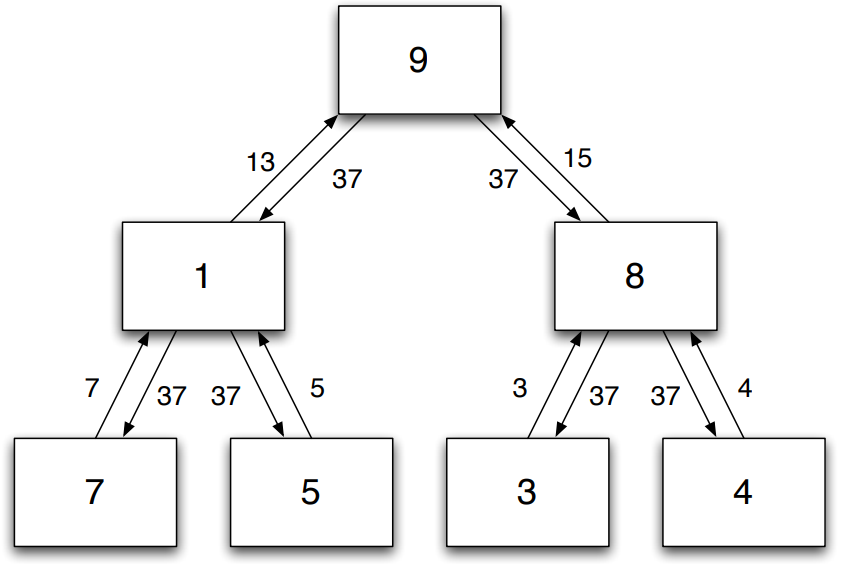
\includegraphics[scale=0.5]{AllReduce.png}
		\captionof{figure}{AllReduce operation. Initially, each node holds its own value. Values are passed up the tree and summed, until the global sum is obtained in the root node (reduce phase). The global sum is then passed back down to all other nodes (broadcast	phase). At the end, each node contains the global sum.}
	\end{minipage}
	\item \textbf{Centralized storage} Centralized storage is used for topologies where a single "master" or "server" node is in the center, and many "slave" or "client" nodes communicate only with this master node. A practical implementation of this is the Parameter Server paradigm (PS). Each Parameter Server keeps a shard of the global model parameters as a key-value store. Each client communicates with the Parameter Server to read / update the parameters. \\
	An advantage is that all model parameters (within a shard) are in a global shared memory, which makes it easy to inspect the model. A disadvantage is that the Parameter Servers can form a bottleneck, because they're handling all communication. To partially alleviate this issue, the techniques mentioned under "Bridging computation and communication" are used.
	\item \textbf{Decentralized storage} In contrast to centralized storage, in decentralized storage every worker maintains its own local view of the parameters, and the workers communicate directly with each other. An example implementation is a peer-to-peer network where every machine broadcasts everything to all other machines. To reduce the amount of communication between all workers, Sufficient Factor Broadcasting (SFB)\cite{Li13}) was proposed. It decomposes the parameter matrix into so-called sufficient factors, i.e. 2 vectors that are sufficient to reconstruct the update matrix. SFB only broadcasts the sufficient factors and lets the workers reconstruct the updates.\\
	An advantage is that, with SFB, decentralized storage is relatively communication-efficient. In addition, there is no centralized bottleneck, making it more scalable.
\end{itemize}










\subsection{Currently used implementations}
This section first shows some generic implementations for distributed systems. These are often used as the foundation for distributed Machine Learning systems. Additionally, several domain-specific implementations are available. For the latter one, the most popular implementations are described, including Distributed Ensemble Learning, Parallel Synchronous SGD, and Parameter Servers.

\subsubsection{Generic distributed system frameworks}
Distributed system have already been implemented in the industry to solve the problem of companies possessing massive amounts of data that they want to be able to query and analyze. These frameworks largely rely on the fact that it is cheaper
to have multiple servers, each of them with a relatively small storage capacity and computing power, rather than having one expensive large server.

\paragraph{The frameworks}
The basis of existing frameworks is based on the Google File System\cite{Ghem03}. The \textit{Google File System} or \textit{GFS} is the system that is used within Google to handle all the Big data needs within the company. It splits all the data that is uploaded to the cluster up into chunks, which are then split over the "chunk servers" in the node, and replicated a predefined number of times (usually 3) in order to guarantee that the data is not lost when a server fails. The
data on the chunk servers can then be accessed by a user by contacting the master, which knows exactly on which servers each chunk is saved.\cite{Ghem03} The data and work-flow is described in figure \ref{GFS_Architecture} below.

\begin{figure}
  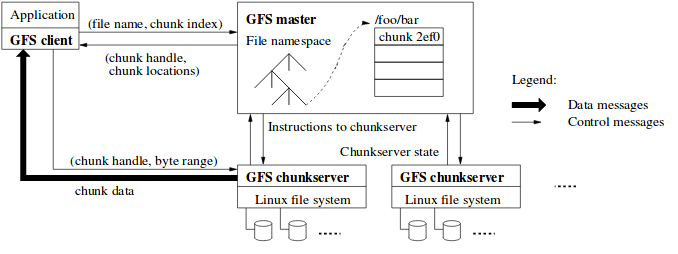
\includegraphics[width=\textwidth]{GFS_Architecture.png}
  \caption{Google File System architecture\cite{Ghem03}}
  \label{GFS_Architecture}
\end{figure}

The GFS architecture that was described in its paper by Google was adapted into an open-source solution called Hadoop \cite{Shv10}. Hadoop was developed mainly by Yahoo!, distributed as an Apache project and functions essentially the same as GFS. There are only minor differences with GFS such as the naming of certain entities and the chunk size. A typical use case of adding a file to the Hadoop File System (HDFS) is show in figure \ref{Hadoop_usecase} below.

\begin{figure}
  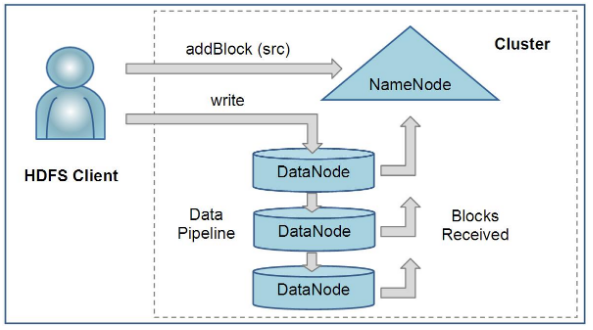
\includegraphics[width=\textwidth]{Hadoop_use_case.png}
  \caption{The data flow when adding a file to the HDFS\cite{Shv10}}
  \label{Hadoop_usecase}
\end{figure}

\paragraph{Uses of the frameworks}
The storage framework highlighted above, is the most-common file-system that empower Big Data implementations today. These implementations are frameworks such as MapReduce and the Apache Spark engine.

\paragraph{MapReduce}
MapReduce is a new framework for processing data and was developed by Google\cite{Dean04} in order to process data in a distributed setting. Firstly, in the \textit{map phase} all data is split into tuples (called key-value pairs). Then, during the shuffle phase, these key-value pairs are shuffled and passed to the \textit{reduce phase} in which a calculation (often an aggregation) is performed on them to generate the a single output value. The main benefit of this framework is that the data can be distributed across a large amount of machines (which are using for example GFS or HDFS). Additionally, instead of communicating the data between the nodes, the program is communicated between the nodes which is magnitudes smaller and more efficient to pass around. A general overview of the execution of a map-reduce problem is given in figure \ref{mapreduce_execution}.

\begin{figure}
  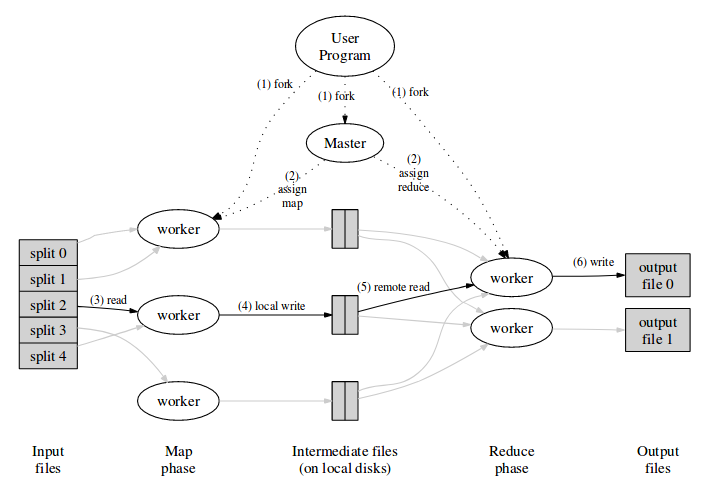
\includegraphics[width=\textwidth]{mapreduce_execution.png}
  \caption{Overview of the execution of a mapreduce problem\cite{Dean04}}
  \label{mapreduce_execution}
\end{figure}

Furthermore the MapReduce framework is similar to the \textit{Bulk-Synchronous processing (BSP)} style which is a little older. However, there are some differences as the MapReduce framework does not allow communication between nodes in the map phase, but only allows communication during the shuffle phase, in-between the mapping and reduce phase\cite{Pace12}.\\
Since BSP and Map-reduce are so similar, peope have worked on transforming BSP tasks into MapReduce tasks. Goodrich et al.\cite{Goo11} has shown that all BSP programs can be converted into MapReduce programs and other researchers have gone as far as to say that all MapReduce task are so similar to BSP tasks that, because BSP has a more theoretical basis, all tasks should be modeled as BSP tasks but implemented using the Map-reduce framework in order to gain the speed of MapReduce and the correctness of BSP\cite{Pace12}.

\paragraph{Apache Spark}
Like MapReduce, Apache Spark is another service built on top of a distributed file system to run programs on a distributed dataset. Spark is an open-source cluster-computing framework that is capable of executing an entire directed acyclic graph of transformations (like mappings) and actions (like reductions) fully in memory\cite{Sparkwebsite}. This is contrast to MapReduce, that forces the programmer to first use a mapping phase and then a reduce phase. This way, Spark is a lot faster than MapReduce because when, for example, 2 mapping phases are needed, 2 MapReduce tasks need to be executed which both require to write all (intermediate) data to the disk. Spark on the other hand can keep all the data in-memory which saves expensive writes to the disk, but needs to take additional steps to prevent losing processed data when there's a power outage.\\

The way in which Spark solves this problem is by using \textbf{RDDs} (Resilient Distributed Datasets). These datasets are read-only and new ones can only be created from data stored on the disk, or transforming existing RDDs\cite{Zaha12}. The Resilient part comes into play when the data is lost. Each RDD has a lineage graph, which shows what transformations have been executed on it. This means that once some data is lost, Spark can trace the path that RDD has followed by using the lineage graph and recalculate any lost data. It is important that the lineage graph does not contain any cycles, i.e. is a Directed Acylic Graph (DAG), because otherwise the data cannot be recovered as Spark will run into an infinite loop.

\begin{figure}
  \begin{center}
    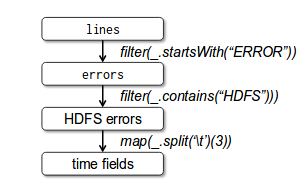
\includegraphics[scale=0.5]{Lineage_graph.png}
  \end{center}
  \caption{Example of the lineage graph of an RDD\cite{Zaha12}}
  \label{lineagegraph}
\end{figure}

With the rising popularity of applied machine learning in many industries, a variety of domain-specific frameworks have been developed that have distribution models tailored towards ML. In this section, we summarize the characteristics of the most popular implementations.

\paragraph{Distributed ensemble learning}
Many frameworks already exist for the development of machine learning models. However, they often have limited support for distributed training, even though they are fast and effective when used on a single machine or high-bandwidth cluster. One way to achieve distribution with these frameworks is through training separate model instances for disjoint subsets of the available data. At prediction time, the outputs of those instances can then be combined through standard ensemble model aggregation\citep{Opitz1999}.
Models that follow this strategy are not dependent on any specific library. They lend themselves well to execution that uses standard distributed systems frameworks. The training process involves executing the individual model trainings on a number of independent machines in parallel. Neither orchestration nor communication are necessary once training has started. Training on $m$ machines with $m$ disjoint subsets of the dataset results in $m$ different models that are serialized somewhere. Each of these can have separate parameters, hyperparameters, and layer architecture. At prediction time, the trained model instances can then all be deserialized and run on new data. This can once again happen in a distributed fashion, through data- and/or model-parallelism.
One large drawback is that this method is dependent on proper subdivision of the training data. If large biases are present in the training sets of some of the models, those instances could have a negative overall effect at prediction time. If the data is divided manually, it's important to ensure independence and indentical distribution. If, on the other hand, the dataset is inherently divided and distributed, this is not quite as straightforward.
There's a large number of existing frameworks available for this method, as any machine learning framework can be used. Some popular implementations are Tensorflow\citep{Tensorflow2015}, MXNet\citep{MXNet2015} and PyTorch\citep{PyTorch2017}. Further analysis of these frameworks is out of scope.

\paragraph{Parallel synchronous SGD}


\subparagraph{Tensorflow \& Baidu AllReduce \citep{BaiduAllReduce2017}}

uses common high performance compute technology (mainly Message Passing Interface (MPI) and its AllReduce operation) to iteratively run SGD model training on separate minibatches of the training data. AllReduce is used to, after each operation, apply each of the workers’ gradients onto the last common model state, and then propagate the result of that operation back to each worker. This is an inherently synchronous process, blocking on the result of each workers’ training iteration before continuing to the next.
Baidu includes a further optimization from \citet{Patarasuk2009} in this process called a Ring AllReduce to reduce the required amount of communication for executing the AllReduce operation. Whereas the naive approach to AllReduce (sending all workers’ state to a central node, which executes the reduction and sends back the result to each worker) would scale in bandwidth linearly with the number of nodes, the Ring AllReduce approach would avoid this by connecting each node only with one neighbor for receiving data, and one neighbor for sending data to. Each node would then execute a reduction on a subset of the reduced data array and forward the result of that to the next node, as long as necessary until each subset of the array has a fully reduced result available on one node. The results are then cycled through the ring step by step, until each node has each subset of the result available to it. Each communication step can be parallellized (utilizing all available bandwidth and putting the bottleneck of communication time at the latency of the slowest link between neighbor nodes) without risk of contention and related efficiency losses.
Baidu claims linear speedup when applying this technique to train deep learning networks. However, it has only been demonstrated on relatively small clusters (5 nodes each, though each node has multiple GPUs that communicate with each other through the same system). Also, although not explicitly mentioned, it is likely that their experimental setup makes use of high bandwidth links between each node, as opposed to the commodity machine approach that many other frameworks offer. The approach lacks fault tolerance by default, as no node in the ring can be missed. This could be counteracted using redundancy (at cost of efficiency), but if not done, the scalability of this method is limited by the probability that every node is available. This can be high when using large numbers of commodity machines and networking to facilitate large datasets.
The system has been integrated into Tensorflow as an alternative to its parameter server-based approach (described below).

\subparagraph{Horovod\citep{Horovod2018}}

takes a very similar approach to that of Baidu and its custom Tensorflow MPI module: it adds a layer of AllReduce-based MPI training to Tensorflow. One difference is that Horovod uses the NVIDIA Collective Communications Library (NCCL) for increased efficiency when training on (Nvidia) GPUs. This also enables use of multiple GPUs on a single node. Data-parallelizing an existing Tensorflow model is relatively simple (a few lines of code need to be added), after which the model can be optimized through synchronous SGD in the same Ring AllReduce-based manner as proposed by Baidu. When benchmarked on Inception v3\citep{Szegedy2015} and ResNet-101\citep{He2015} using 128 GPUs, efficiency of distribution is about 88\%, compared to about 50\% in Tensorflow's parameter server approach.
However, Horovod lacks fault tolerance (much like in Baidu's approach), and the same scalability concerns therefore arise.

\subparagraph{Caffe2}

(primarily maintained by Facebook) distributes ML (data-parallel) through, once again, AllReduce. It does this using NCCL between GPUs on a single host, and custom code between hosts that uses Facebook's Gloo library, which abstracts over multiple transports (e.g. TCP/IP or InfiniBand). Facebook uses Ring AllReduce (which offers better bandwidth \& parallelism guarantees) but also recursive halving and doubling (a divide-and-conquer approach that offers better latency guarantees). According to their paper, performance is improved in latency-limited situations such as for small buffer sizes and large server counts. The end result of Facebook’s approach is that they can train ResNet-50\citep{He2015} in the span of 1 hour\citep{Goyal2017}, achieving linear scaling with the number of GPUs, at 90\% efficiency and measured up to 352 GPUs. However, once again no fault-tolerance is present, which raises some questions on the topic of scalability.

\subparagraph{CNTK}

offers multiple modes of data-parallel distribution, a subset of which (the synchronous ones) use the Ring AllReduce tactic previously described, with the same tradeoff (achieving linear scalability at expense of fault tolerance). Two innovations are offered by the library:

1-bit stochastic gradient descent (\citet{Seide2014}) is an implementation of SGD that quantizes training gradients to a single bit per value. This reduces the number of bits that need to be communicated when doing distributed training by a large constant factor.

Block-momentum SGD (\citet{Chen2016}) divides the training set into m blocks and n splits. Each of n machines trains a split in each block. The gradients calculated for all splits within a block are averaged to arrive at the weights for the block. The block updates are then merged into the global model, while applying block-level momentum and learning rate.

When benchmarked on a Microsoft speech LSTM, average speedups of 85\%+ are achieved for small numbers of GPUs (up to 16), but scalability drops significantly (below 70\%) when scaling past that \footnote{Direct comparison of this number to the other synchronous frameworks' results is somewhat unfair, as the dependency structure of an LSTM is significantly different than that of an ordinary DNN due to the introduction of temporal state.}.


\paragraph{Parallel asynchronous SGD \& Parameter Servers}

\subparagraph{DistBelief \citep{DistBelief2012}}

is one of the early practical implementations of large-scale distributed learning, developed by Google. They encountered the limitations of GPU training, and built DistBelief to counteract them. DistBelief supports data- and model-parallel training on tens of thousands of CPU cores (though GPU support was later introduced as well\citep{Tensorflow2016}). At the time of the paper's writing, it was used to successfully train models 30x larger than reported in preceding literature.
 
At the time, Google also evaluated solutions based on MapReduce\citep{MapReduce} and GraphLab\citep{GraphLab}. MapReduce ”was ill-suited for the iterative computations inherent in deep network training”. GraphLab “would not exploit computing efficiencies available in the structured graphs typically found in deep networks”. This led the company to develop a domain-specific alternative instead.

To achieve efficient model-parallelism, DistBelief exploits the graphical nature of neural networks. Machines each execute the training of a part of the model, which can span subsets of multiple layers. Communication is only required at those points where a node’s output is used as the input of a node trained by another machine. To define a DistBelief model, “[t]he user defines the chilimbiomputation that takes place at each node in each layer of the model, and the messages that should be passed during the upward and downward phases of computation.” Partitioning of the model across a cluster is transparent and requires no structural modifications. Efficiency of a given partitioning, however, depends on the model’s connectivity structure and computational needs, and requires careful design. Locally connected models, for example, lend themselves for model parallelism, because of limited cross-partition communication. Fully connected models, on the other hand, have more substantial cross-partition dependencies and are therefore harder to efficiently distribute through DistBelief.

To further parallelize model training, data parallelism is applied on top of the model parallelism. A centralized sharded parameter server is used to allow each of a set of model replicas (which may internally be model-parallel) to share parameters. DistBelief supports two methods of data parallelism, both of which are resilient to processing speed variance between model replicas, as well as full replica failure. The first method is downpour SGD, an asynchronous alternative to the inherently sequential SGD. Each replica of the model fetches the latest model parameters from the parameter server every $n_{fetch}$ steps, updates these parameters in accordance with the model, and pushes the tracked parameter gradients to the parameter server every $n_{push}$ steps. Simple implementations would use $n_{fetch} = n_{push} = 1$, causing it to fetch the parameters before every training iteration, and push the iteration’s gradient once it is available. Communication overhead can be reduced by increasing either or both parameters. Fetches and pushes could also each be executed on a separate thread, which would require only weak synchronization between each other and the training thread.

The downpour SGD algorithm primarily used in DistBelief is resilient to machine failures more than SGD, as it allows training to continue even if some model replicas are offline. The optimization process itself, however, becomes less predictable due to parameters that are out of sync on the model replicas or between shards of the parameter server. No theoretical guarantees or citations are offered to support the robustness of this approach, yet the authors “found relaxing consistency requirements to be remarkably effective.” Tactics that contribute to robustness are the application of adaptive learning rates through AdaGrad\citep{Duchi2011} and “warmstarting “the model through training a single model replica for a while before scaling up to the full number of machines. The authors make note of not having stability issues after applying these.
A second method of parallelization is distributed L-BGFS. This makes use of an external coordinator process that divides training work between model replicas, as well as some operations on the parameters between the parameter server shards.

The shards of the parameter server each hold a fraction of the total parameter space of the model being trained. The model replicas pull the parameters from all shards; each parallelized part of the model only retrieves those parameters that it needs.

Performance improvements are high but very expensive in terms of CPU hours: while the best speedup (downpour SGD with AdaGrad) achieved an 80\% decrease in training time on ImageNet, this was achieved using more than 500 machines and more than 1000 CPU cores. However, DistBelief did not support distributed GPU training at the time of \citet{DistBelief2012}, which could reduce the required resources quite significantly and is in fact used in almost all other implementations mentioned in this section.

\subparagraph{Tensorflow \citep{Tensorflow2015}\citep{Tensorflow2016}}

is the evolution of DistBelief, in the sense that it was developed to replace DistBelief within Google, and borrows both concepts and experience from it. It also applies subsequent optimizations to the parameter server model, like \citet{Chilimbi14} and \citet{Li2014Comms}\citep{Li2014Scaling}. By "both simplifying and generalizing [DistBelief]"\citep{Tensorflow2016}, the Tensorflow developers intend to cater to a wider variety of ideas.

TensorFlow represents both model algorithms and state as a dataflow graph, execution of which can be distributed. This facilitates different parallelization schemes that can take e.g. state locality into account. The level of abstraction of the dataflow graph is that of mathematical operations on tensors (i.e. $n$-dimensional matrices), as opposed to DistBelief, which abstracted at the layer level. Consequently, defining a new type of neural network layer in Tensorflow requires no custom code - it can be represented as a subgraph of a larger model, composed of simpler math operations.

A Tensorflow model is first defined as a symbolic dataflow graph. Once this graph has been constructed, it is optimized and then executed on the available hardware. One advantage of this model is that it allows Tensorflow to tailor its execution strategy towards the types of devices available to it. When working with e.g. GPUs or TPUs (Tensor Processing Units\citep{TPU2017}), Tensorflow can take into account the asynchronicity and intolerance to branching that is inherent to these devices, without requiring any changes to the model itself.

\citet{Shaohuai2017} show Tensorflow achieving sub-40\% efficiency on 4-node, InfiniBand-connected cluster training of ResNet-50\citet{He2015}, and about 75\% efficiency on GoogleNet\citep{Szegedy2014}. 


\subparagraph{MXNet \citep{MXNet2015}}

uses a strategy very similar to that of Tensorflow: models are represented as dataflow graphs, which are executed on hardware that is abstracted away, and coordinated using a parameter server. MXNet, however, also supports imperative definition of dataflow graphs as operations on n-dimensional arrays (which simplifies the implementation of certain kinds of networks).

MXNet's parameter server is used in the form of an abstraction: the KVStore. The KVStore supports pushing key-value pairs from a device to the store, and pulling the current value of a key from the store. There is support for user-defined update logic that is executed when a new value is pushed, and for multiple consistency models enforced by the KVStore (currently limited to sequential and eventually consistent execution). The KVStore is a two-tier system: updates by multiple threads and GPUs are merged on the local machine before they're pushed to the full cluster.

The KVStore abstraction theoretically enables the implementation of (stale-)synchronicity, although only an asynchronous implementation is present at the time of writing. 

On a small cluster (10 machines), MXNet achieves super-linear speedup compared to a single machine when training GoogleNet\citep{Szegedy2014} with more than 10 passes over the data. \citet{Shaohuai2017}, however, show its efficiency to dip to 65\% when trained on more than one machine using GoogleNet\citep{Szegedy2014}, and 50\% using ResNet-50\citet{He2015}. Performance here was evaluated on a single epoch (after warm-up) on nodes linked using Infiniband, but it does suggest that \citet{MXNet2015}'s achieved performance needs some tuning. The paper lacks information on the exact process required.

\subparagraph{CNTK}

again uses a strategy similar to MXNet and Tensorflow. It makes use of dataflow graphs for model definition. Instead of the integrated parameter server approach of the other libraries, however, CNTK uses a separated parameter server called Multiverso, which can also be used by other frameworks.

Performance (both on a single node and on a cluster) seems to be the main factor at which CNTK attempts to differentiate itself. \citet{Shaohuai2017} show CNTK achieving very competitive results of about 75\% efficiency on ResNet-50\citep{He2015} in a 4-node, InfiniBand-connected cluster configuration, outperforming both Tensorflow and MXNet by a significant margin. 

\paragraph{Parallel stale-synchronous SGD}

\subparagraph{Petuum \citep{Xing2013}}

aims to provide a generic platform for any type of machine learning (as long as it is iteratively convergent) on big data (terabytes/petabytes) and big models (hundreds of billions of parameters). It supports data- and model-parallelism. The Petuum approach exploits ML’s error tolerance, dynamic structural dependencies, and non-uniform convergence in order to achieve good scalability on large datasets and models. This is in contrast to e.g. Spark (focusing on fault tolerance \& recovery) and GraphLab (focusing on consistency), which can still be important to ML, but don't inherently have a positive performance impact. The platform uses stale synchronicity to exploit error tolerance (since a minor amount of staleness will have minor effects on convergence), dynamic scheduling policies to exploit dynamic structural dependencies (which helps minimize parallelization error and synchronization cost) and unconverged parameter prioritization to take advantage of non-uniform convergence (by reducing computational cost on parameters that are already near optimal). 

Petuum uses the parameter server model (as proposed by \citet{DistBelief2012}) to keep track of the parameters of the model being trained. The parameter server is also responsible for maintaining the staleness guarantees. In addition, it exposes a scheduler that lets the model developer control the ordering of parallelized model updates.

The programming model that Petuum used is different to that of DistBelief in one core way: data- and model-parallelism operate at the same tier. Whereas in DistBelief model-parallelism is managed inside model shards, and each model replica operates on the parameter server as a single entity, Petuum instead has both model and data slices interact with the parameter server directly, and requires the user to define some central update logic if model-parallelism is involved. This allows slightly more programmer control.

When developing a model using Petuum, developers have to implement at least one method, named push, which is responsible for each of the parallelized model training operations. Its implementation should pull the model state from the parameter server, run a training iteration, and push a gradient to the parameter server. Petuum by default automatically manages the scheduling aspect and the parameter merging logic, so that data-parallel models don’t require any additional operations. If you want model-parallelism, however, you need to also implement the schedule method (which tells each of the parallel workers which parameters to train) and the pull method (which defines the aggregation logic for each of the parallelly generated parameter gradients).

Petuum provides an abstraction layer that also allows it to run on systems using YARN and HDFS, which simplifies compatibility with pre-existing clusters. 


\paragraph{Parallel hybrid-synchronous SGD}

Both synchronous and asynchronous approaches have some significant drawbacks, as is explored by \citet{ChenJianmin2016}. A few frameworks attempt to find a middle ground instead that combines some of the best properties of each model of parallelism, and diminishes some of the drawbacks.

\subparagraph{MXNet-MPI \citep{Mamidala2018}}

takes an approach to distributed ML (using a modified version of MXNet as a proof of concept) that combines some of the best aspects of both asynchronous (parameter server) and synchronous (MPI) implementations. The idea here is to use the same approach as described in the MXNet section, but instead of having single workers communicate with the parameter server, to cluster those workers together into groups that internally apply synchronous SGD over MPI/AllReduce. This has the benefits of easy linear scalability of the sync MPI approach, and fault tolerance of the asynchronous parameter server approach.



\subsubsection{Current challenges}
\paragraph{Performance}

A trade-off that’s seen frequently is the reduction of wall-clock time at the expense of total processing time (i.e. decreased efficiency). When compute resources are affordable enough, many real-world use cases of machine learning benefit most from being trained rapidly. The fact that this often implies a large multiple in total compute resources (and the associated energy consumption) is not as important, as long as a model saves more money than it costs to run.  A good example of this is found in \citet{DistBelief2012}, where wall clock time speedup factors are achieved by increasing the number of machines quadratically or worse. It still delivered Google competitive advantage for years. Distributed use of GPUs, as in Tensorflow, has better properties, but often still exhibits efficiency below 75\%.
These performance concerns are much less severe in the context of synchronous SGD-based frameworks, which often do achieve linear speedups in benchmarks. However, most of these benchmarks test at most a few hundred machines, whereas the scale at which e.g. DistBelief is demonstrated can sometimes be two orders of magnitude larger. The reason for this is unclear, although it might be related to the fault tolerance concerns mentioned below. Synchronous frameworks also benefit more from high-bandwidth links such as InfiniBand, due to the fact that all nodes' communication is synchronized. However, those are expensive (with costs running up to thousands of euros for even a cheap switch) and can't practically be used in large footprint clusters (e.g. in multiple datacenters) due to wiring and latency constraints.

\paragraph{Fault tolerance}

Synchronous AllReduce-based approaches seem to scale significantly better than the parameter server approach (up to a certain cluster size), but suffer from a lack of fault-tolerance: failure of a single machine blocks the entire training process. At smaller scales, this might still be a manageable problem. However, past a certain number of nodes the probability of any node being unavailable becomes high enough to result in near-continuous stalling. Common implementations of these HPC-inspired patterns, such as MPI and NCCL, lack fault-tolerance completely. Although there are efforts to counteract some of this, production-ready solutions are lacking. Some of the described implementations allow for checkpointing to counteract this, but a lot of work is necessary to enable true fault-tolerance, as is described in \citet{Amatya2017}. It is also possible to reduce the probability of failure for each individual node, but this requires very specific hardware that is expensive (e.g. highly stable datacenter cooling or Infiniband networks) and not generally available on commodity cloud platforms.
Asynchronous implementations do not suffer from this problem as much. They are designed to explicitly tolerate straggling and failing nodes, with only minimal impact on training performance. The question for ML practitioners, then, is whether they prefer performance or fault tolerance, and whether they are constrained by either one. Hybrid approaches even offer a way to customize these characteristics, although they are not frequently found in use yet. It would be interesting to see whether an even better approach exists, or whether there is an efficient way to implement fault-tolerant AllReduce.

\paragraph{Privacy}

There are scenarios in which it is beneficial or even mandatory to isolate different subsets of the training data from each other. The furthest extent of this is when a model needs to be trained on datasets that each live on different machines/clusters, and may under no circumstance be co-located or even moved.
One interesting approach to training models in a privacy-sensitive context is the use of a distributed ensemble model. This allows perfect separation of the training data subsets, with the drawback that a method needs to be found that properly balances each trained model's output for an unbiased result.
Parameter server-based systems could also be useful in the context of privacy, as the training of a model can be separated from the training's result. However, this assumes that no sensitive properties of the underlying data leak into the model itself, which is not always easy to prove.
Finally, it is possible to introduce statistical noise into each subset of the training data, with the intention of rendering its sensitive characteristics unidentifiable to other parties. \citet{Bal12} touches on this subject, but makes it clear that the amount privacy in this scenario is dependent on the amount of statistical queries required to learn the dataset. This puts an upper bound on usefulness of the model itself.
In conclusion, it is highly unlikely that perfect privacy is possible, but current frameworks do not offer much support for even basic variants. It could be interesting to answer whether there's a generic way to facilitate distributed privacy, which could then be integrated into the frameworks that are being used.

